\documentclass{standalone}
% pdflatex EKF_schema.tex
% magick -density 300 KF_schema.pdf -quality 90 -resize 640x640 KF_schema.png
\usepackage{tikz}
\usetikzlibrary{arrows.meta}
\usepackage{amsmath}
\DeclareMathOperator{\sign}{signo}

\begin{document}

% Models for time series 
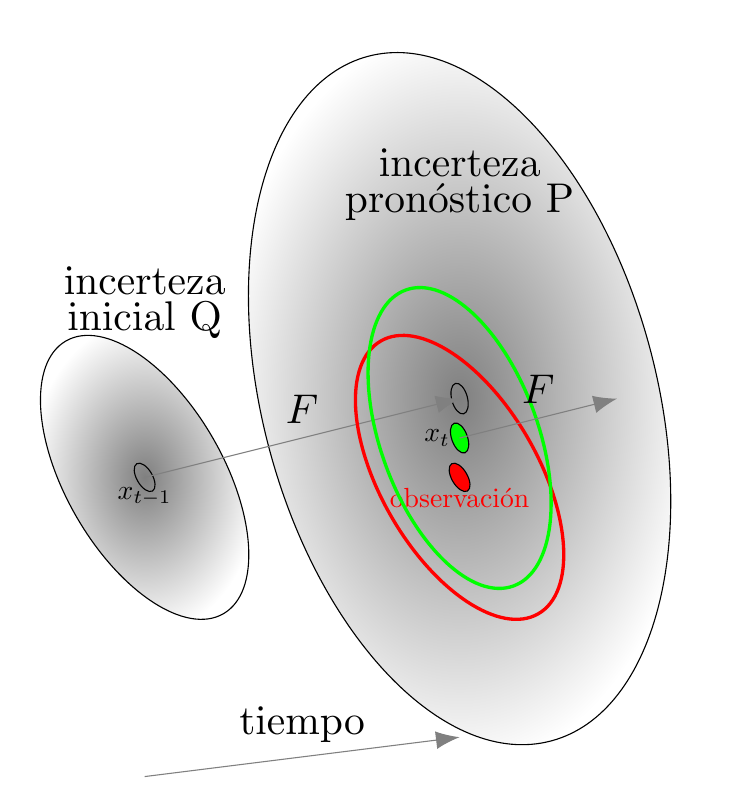
\begin{tikzpicture}


  \shade[inner color=gray, outer color=white, draw=black] (3,3) circle [x radius=1, y radius=2, rotate=30];

  \draw[draw=black] (3,3) circle [x radius=0.1, y radius=0.2, rotate=30]   node[below, scale=1]{$x_{t-1}$};

    
  \shade[inner color=gray, outer color=white, draw=black] (7,4) circle [x radius=2.5, y radius=4.5, rotate=15];
  \draw[draw=black] (7,4) circle [x radius=0.1, y radius=0.2, rotate=15];
  
  \node[scale=1.5, black] at (3,5.5)  {incerteza};
  \node[scale=1.5, black] at (3,5)  {inicial Q};

  \draw[gray, -{Latex[length=3mm]}] (3,3)  -- (7,4)
  node[align=center, above, pos=0.5, scale=1.5, black] {$F$};

  \node[scale=1.5, black] at (7,7) {incerteza};
  \node[scale=1.5, black] at (7,6.5) {pronóstico P};

  \draw[gray, -{Latex[length=3mm]}] (3,-0.8)  -- (7,-0.3)
  node[align=center, above, pos=0.5, scale=1.5, black] {tiempo};

  \draw[fill=red] (7,3) circle [x radius=0.1, y radius=0.2, rotate=30];
  \draw[draw=red, very thick] (7,3) circle [x radius=1, y radius=2, rotate=30] node[below, scale=1, red] {observación};

  
  \draw[fill=green] (7,3.5) circle [x radius=0.1, y radius=0.2, rotate=20]
  node[below, scale=1, left]{$x_t$};
  \draw[draw=green, very thick] (7,3.5) circle [x radius=1, y radius=2, rotate=20];
  

  \draw[gray, -{Latex[length=3mm]}] (7,3.5)  -- (9,4)
  node[align=center, above, pos=0.5, scale=1.5, black] {$F$};
  
\end{tikzpicture}


\end{document}
